\chapter{Proposed Models}\label{Chapter:proposals}

The biggest criticism of deep learning is its overt dependence on voluminous data which has lead many researchers to argue that deep networks are only good at finding pattern recognition in training distribution and therefore conform to the basic tenet of statistical machine learning that train and test data should come from the same distribution. Deep neural networks therefore are still poor at zero shot generalization to test data which despite coming from the same \lq rule space {}\rq\ don't follow the exact same distribution as training data (find a good example here). Human reasoning on the other hand is governed by a rule based systematicity which leads us to learn complex concepts from small samples which leads to zero shot generalization (example ).

\cite{Liska2018} using lookup tables (section \ref{datasets:lt}) as the testbed tried to asses the ability of a RNN network (more specifically a 60 unit LSTM followed by a 10 unit sigmoid layer) to search for compositional solution to the lookup table task. Lookup tables exhibit functional nesting and therefore a model that can find a compositional solution from the search space of all possible solutions is more likely to zero shot generalize to novel compositions. The authors established that by having additional supervision on the weights of hidden state transitions, theoretically a finite-state automata (FSA) can be induced such that the recurrent layers encode the states of this automaton. This FSA can in principle solve the lookup table task upto a finite number of compositions. They further showed that this theoretical setup can achieve zero state generalization on unseen inputs on known compositions i.e. \textit{heldout inputs} (section \ref{lt:splits}).

However when trained purely on input/output mappings without this additional supervision, the authors noted that only a small percentage of networks could converge to a compositional solution (models capable of zero shot generalizing to unseen inputs on known compositions). Additional these small percentage of models also only showed a weak form of composition wherein if for instance t1, t2 are atomic tables, then a composition task t1 t2 is indexed to prompt t1t2, instead of solving in a nested fashion viz. t1(t2(.)). (Get feedback here, see if this is clear)

Motivation for AG - Lake's work as an inspiration should come here, something about learning the trace of a program.\cite{Lake2015}

What is AG?

How AG in seq2seq directly translates to pondering?

\begin{figure}
	\begin{minipage}[t]{\textwidth}
		\ifpdf
		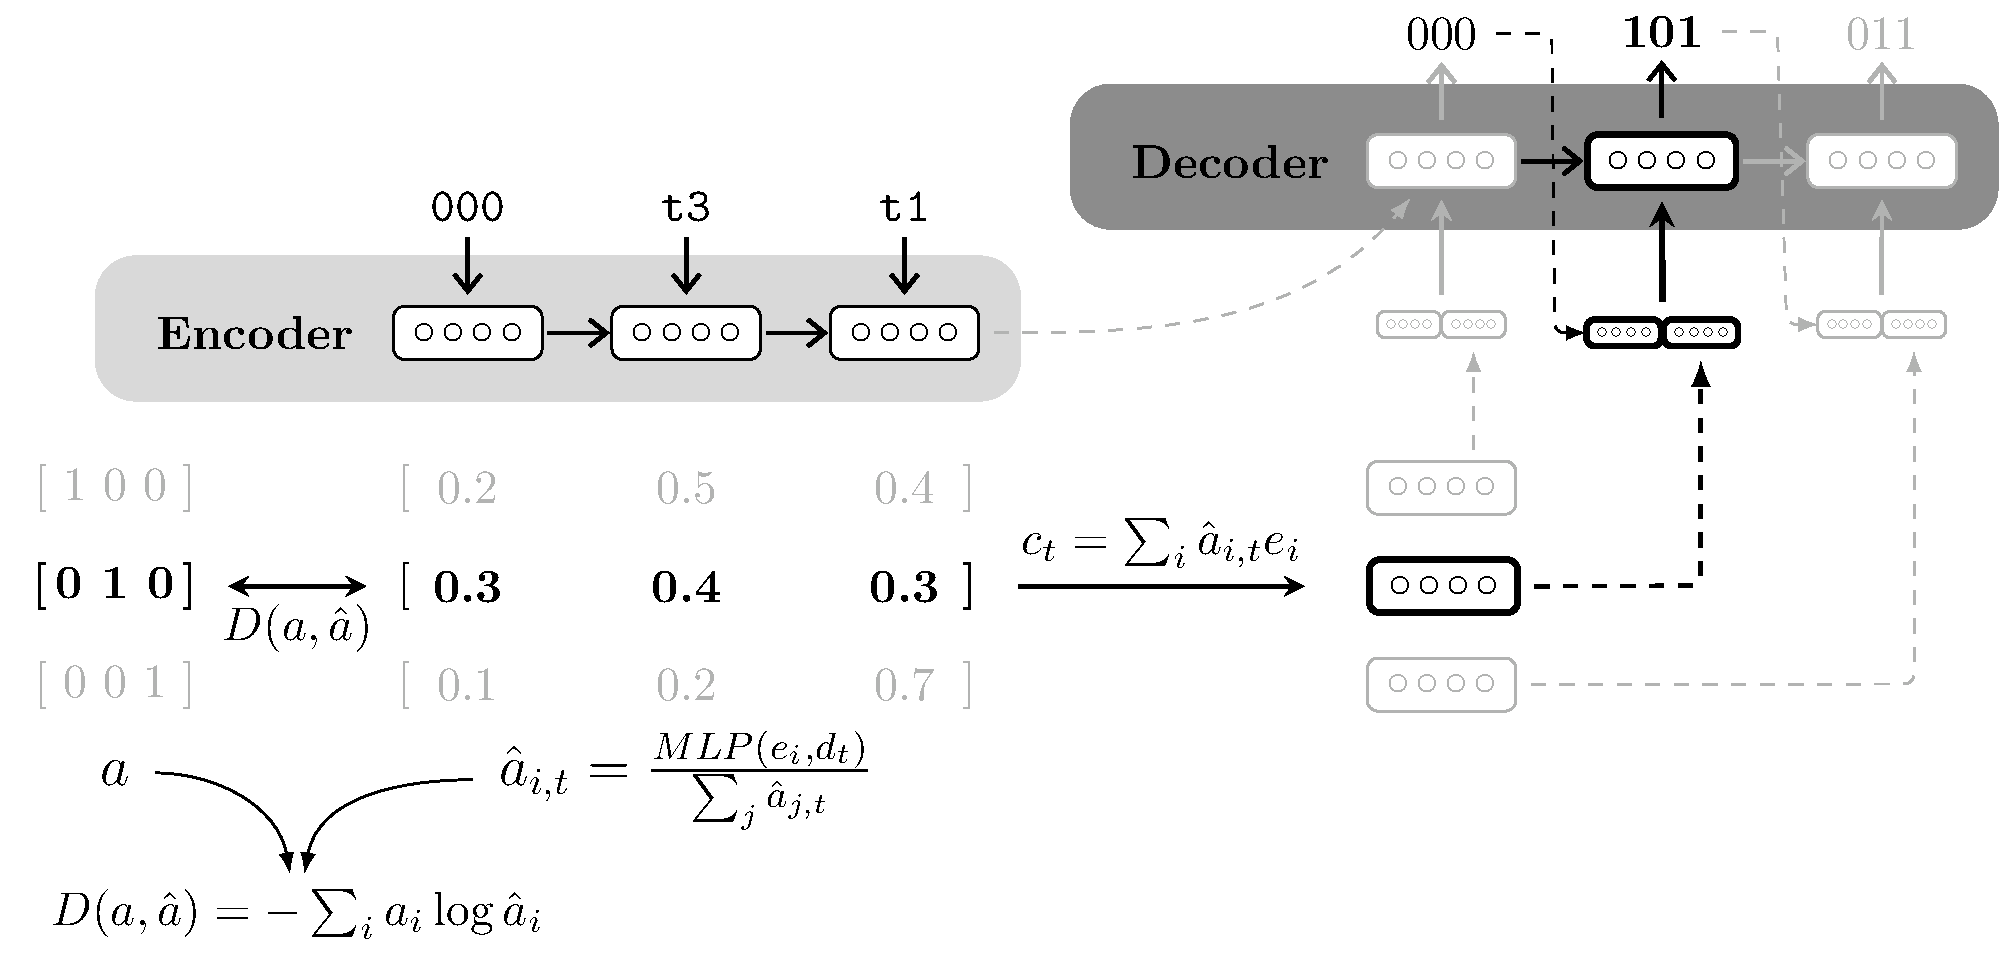
\includegraphics[width=\linewidth,keepaspectratio=true]{./figs/ag-model-pdf}
		\else
		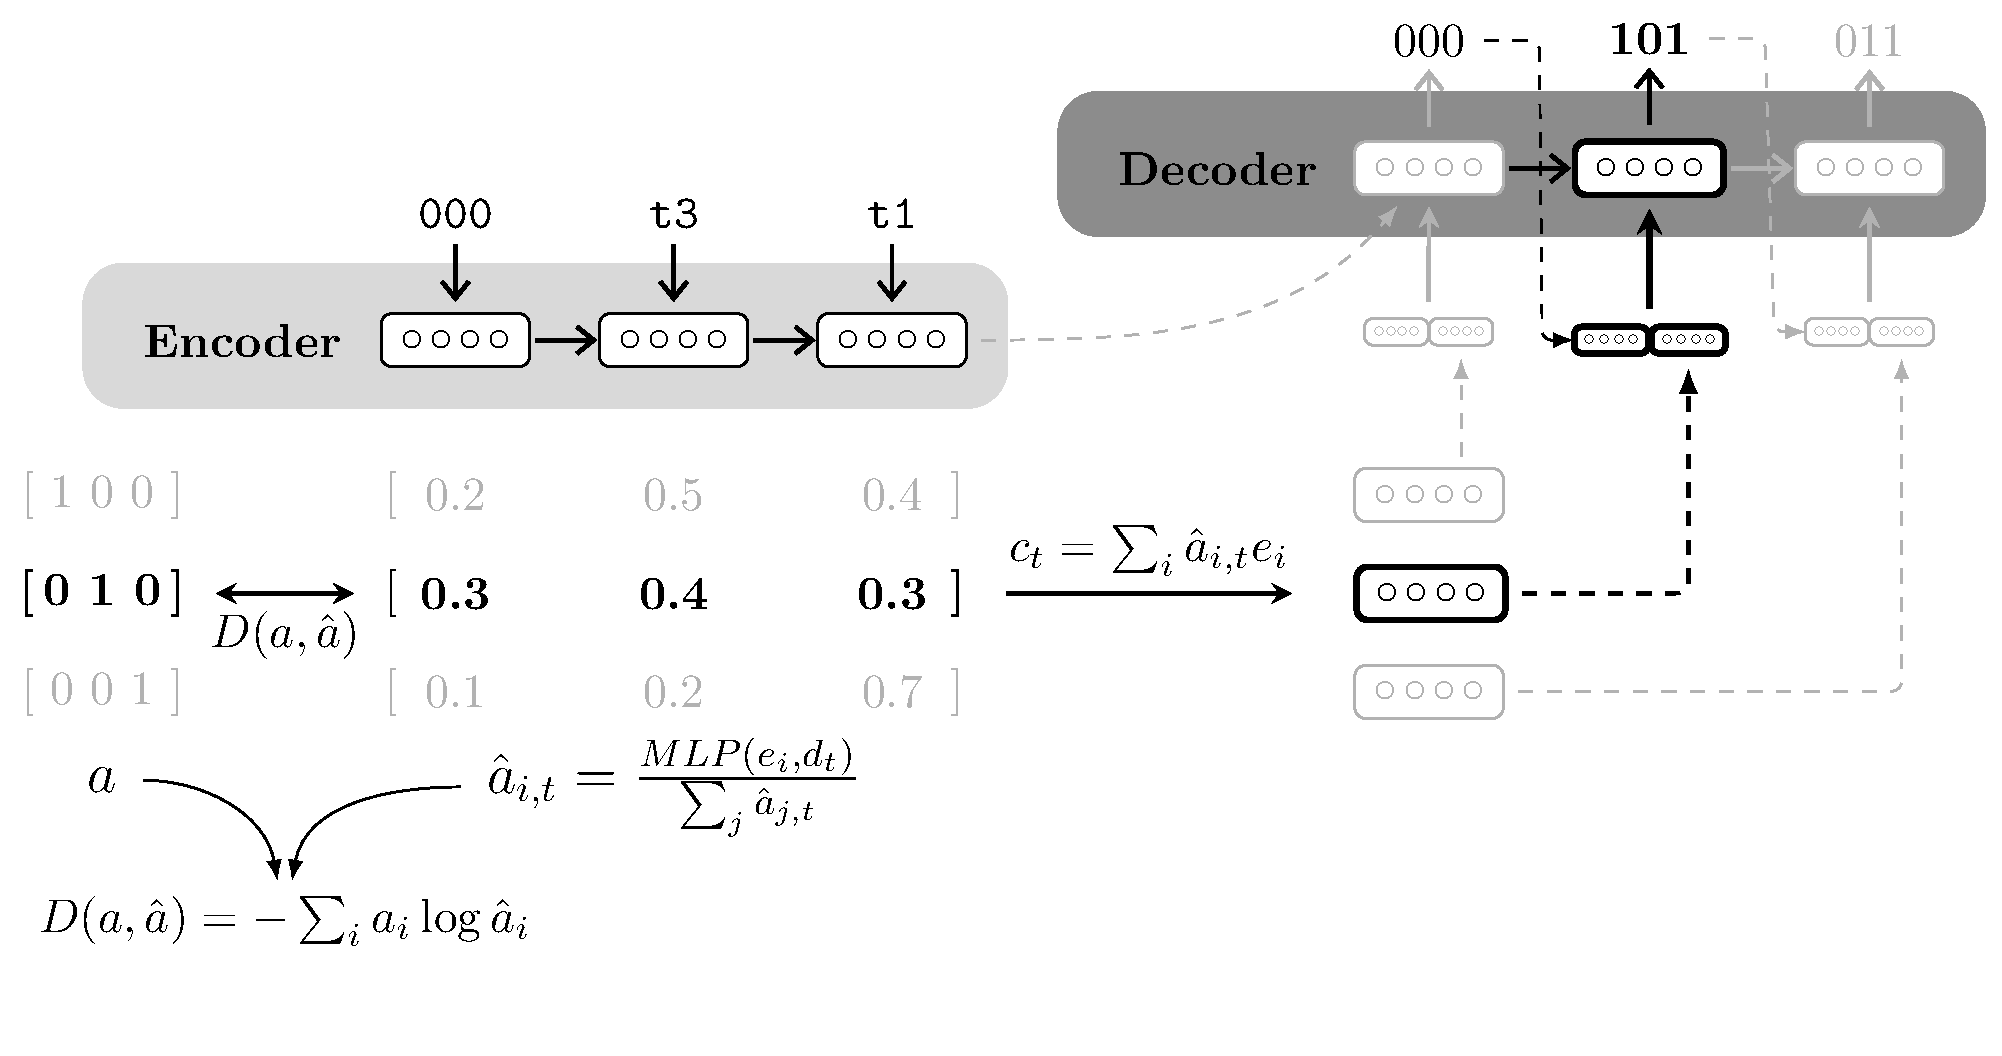
\includegraphics[width=\linewidth,keepaspectratio=true]{./figs/ag-model-eps}
		\fi
		\caption{\small Attentive Guidance}
		\label{pm:ag}
	\end{minipage}
\end{figure}